\documentclass[%singlesided,
               doublesided,
               paper=a4,
               fontsize=10pt
              ]{my-resume}

%% PUBLICATION LIST

\usepackage[backend=biber,style=apa,sorting=ydnt,uniquename=false,isbn=false,maxbibnames=99,url=false,giveninits=true,eprint=false]{biblatex}
\AtEveryBibitem{\clearfield{note}}
\addbibresource{sample.bib}

\usepackage{url}

%%%%%%%%%%%%%%%%%%%%%%%%%%%%%%%%%%%%%%%%%%%%%%%%%%%%%%%%%%%%%%%%%%%%%%%%%%%%%%%%
% set geometry
%%%%%%%%%%%%%%%%%%%%%%%%%%%%%%%%%%%%%%%%%%%%%%%%%%%%%%%%%%%%%%%%%%%%%%%%%%%%%%%%

\setlength\highlightwidth{8cm}
\setlength\headerheight{4cm}            % note that margintop gets added to this value, i.e. the header bar is 5cm
\setlength\marginleft{1cm}
\setlength\marginright{\marginleft}      % needs to be 1.5 times to be actually equal. why?
\setlength\margintop{1cm}
\setlength\marginbottom{1cm}


%%%%%%%%%%%%%%%%%%%%%%%%%%%%%%%%%%%%%%%%%%%%%%%%%%%%%%%%%%%%%%%%%%%%%%%%%%%%%%%%
% FONTS
%%%%%%%%%%%%%%%%%%%%%%%%%%%%%%%%%%%%%%%%%%%%%%%%%%%%%%%%%%%%%%%%%%%%%%%%%%%%%%%%

\RequirePackage{fontspec}
\setmainfont{Carlito}


%%%%%%%%%%%%%%%%%%%%%%%%%%%%%%%%%%%%%%%%%%%%%%%%%%%%%%%%%%%%%%%%%%%%%%%%%%%%%%%%
% COLORS
%%%%%%%%%%%%%%%%%%%%%%%%%%%%%%%%%%%%%%%%%%%%%%%%%%%%%%%%%%%%%%%%%%%%%%%%%%%%%%%%

\colorlet{highlightbarcolor}{lightgray}
\colorlet{headerbarcolor}{black}

\colorlet{headerfontcolor}{white}
\colorlet{accent}{awesome-skyblue}
\colorlet{heading}{black}
\colorlet{emphasis}{black}
\colorlet{body}{black}


%%%%%%%%%%%%%%%%%%%%%%%%%%%%%%%%%%%%%%%%%%%%%%%%%%%%%%%%%%%%%%%%%%%%%%%%%%%%%%%%
% set document
%%%%%%%%%%%%%%%%%%%%%%%%%%%%%%%%%%%%%%%%%%%%%%%%%%%%%%%%%%%%%%%%%%%%%%%%%%%%%%%%


\begin{document}

\name{Alessio Rovere}
\tagline{Ph.D. in Marine Environmental Sciences.\\ Full Professor in physical geography and geomorphology.\\
Access my full CV \href{https://github.com/Alerovere/Resume/blob/main/Resume_AR/Resume_full_ENG.pdf}{here \faExternalLink}\\
\small{Last update: \today}}
\photo[round]{picture.jpg}{\dimexpr \headerheight-\marginbottom}   % make photo exactly match the header with margintop/marginright/marginbottom as margin

\makeheader

\highlightbar{
    \section[\faInfoCircle]{About me}
{\normalsize I am a geoscientist specializing in the evolution of coastal areas. In particular I study coastal dynamics and sea-level changes at various timescales, from millions of years to decades. I am a passionate surfer, wing foiler and scuba diver.}


    \section[\faEnvelopeO]{Contact}
    \email{alessio.rovere@unive.it}
    \location{DAIS. Via Torino 155, Mestre (VE)}
    \homepage{https://avacard.app/Alerovere}{https://avacard.app/Alerovere}
    \github{@Alerovere}{https://github.com/Alerovere}
    \orcid{0000-0001-5575-1168}{https://orcid.org/0000-0001-5575-1168}


    \section[\faShareAlt]{Social}
    \faTwitterSquare \hspace{0.5em} \href{https://twitter.com/alessio_r_}{@alessio\_r\_}\\
    \faInstagram \hspace{0.5em} \href{https://www.instagram.com/alessio_rovere/}{@Alessio\_Rovere}\\
    \faSpotify \hspace{0.5em} \href{https://open.spotify.com/show/1mksP88jgLHqKnndVkEoUq}{Storie di Mare}\\
    \faYoutubePlay \hspace{0.5em} \href{https://www.youtube.com/c/AlessioRovereMarineScience/}{@CoastalScience}\\
    \faLinkedin \hspace{0.5em} \href{https://www.linkedin.com/in/alessio-rovere-591836334}{Alessio Rovere}

    \section[\faBriefcase]{Honorary positions}
     \achievement{\textbf{Since 2024} Honorary Professor, University of Bremen} 
     \achievement{\textbf{Since 2022} External member, MARUM, University of Bremen}
     \achievement{\textbf{04/2014 - 08/2021} Adjunct Associate Research Scientist, LDEO, Columbia University}

    \section[\faPlane]{Visiting periods}
    \achievement{\textbf{2010.} University of Western Australia}
    \achievement{\textbf{2010.} Brunel University, UK}
    \achievement{\textbf{2009-2010.} University of the Aegean, GR}
    \achievement{\textbf{2004.} Universidad de Las Palmas de Gran Canaria (ERASMUS), ES}
    }
\mainbar{
    \section[\faGears]{Work history}
    \job{Since 1/2024}
        {Universitá Ca' Foscari - Venezia (IT)}
        {Full Professor}
        {}
    \job{11/2021 - 11/2024}
        {Universitá Ca' Foscari - Venezia (IT)}
        {Associate Professor}
        {}
    \job{03/2019 - 10/2021}
        {MARUM and University of Bremen \\- Bremen (DE)}
        {Independent research scientist}
        {}
    \job{03/2014 - 02/2019}
        {MARUM, University of Bremen \\ and Leibniz ZMT - Bremen (DE)}
        {Young Investigator Group Leader}
        {}
    \job{02/2012 - 02/2014}
        {Lamont Doherty Earth Observatory, \\ Columbia University - New York (USA)}
        {Postdoctoral research scientist}
        {}
    \job{10/2010 - 12/2016}
        {SEAMap SRL, a Spin-off company \\ of the University of Genoa (IT)}
        {Director (Amministratore Unico)}
        {}
        
    \section[\faMortarBoard]{Education}
    \job{01/2008 - 12/2010}
        {University of Genoa (IT)}
        {Ph.D. in Marine Sciences}
        {European Ph.D. Label}
    \job{01/2008 - 12/2010}
        {University of Genoa (IT)}
        {Master of science }
        {Marine Environmental Sciences}
    \job{01/2008 - 12/2010}
        {University of Genoa (IT)}
        {Bachelor of science}
        {Environmental Sciences}
        
\section[\faSlideshare]{Teaching}
{\normalsize I have been teaching several courses at the University of Bremen and Ca' Foscari University of Venice. I currently teach the courses \textbf{"Coastal hazards (MSc)"} and \textbf{"Physical geography and geomorphology (BSc)"} at Ca' Foscari and the course \textbf{"Sea Level Changes (MSc)"} at the University of Bremen.}

\bigskip

\section[\faGroup]{Mentoring and supervision}
{\normalsize I have mentored \textbf{nine postdoctoral researchers}. Upon leaving my team, several researchers have successfully transitioned to other academic positions or into industry roles. I supervised \textbf{four doctoral students} until the completion of their thesis. I supervised as main or co-supervisor \textbf{twenty one BSc or MSc students} from different European Universities.}
}
\makebody                  
\clearpage

\pagestyle{highlightmain}

% The highlightbar needs to be filled to display mainbar contents correctly in singlesised mode
% For an empty highlightbar, fill with empty space
\highlightbar{

\section[\faGraduationCap]{Research}
{\small My research spans a broad range of geographical areas, focusing on coastal and sea- level changes. I investigate \textbf{modern coastal transformations} in Germany and Ghana. In tropical areas like Moorea, Tahiti, and Fiji, my studies explore the \textbf{interactions between modern coastal processes and coral reef ecological dynamics}. Additionally, I examine \textbf{paleo sea-level variations (from the Holocene to the Pliocene)} in diverse locations such as the Mediterranean, USA, Cape Verde, the Bahamas, Aruba, Curaçao, Bonaire, Madagascar, Bermuda, Argentina, Brazil, Seychelles, South Africa, and Indonesia. My work also entails studying the \textbf{underwater topography of coral reefs} in the Maldives. I employ a variety of methodologies to tackle the complexities of marine and coastal geomorphology at these globally distributed sites. I have led research expeditions to all the aforementioned locations, overseeing logistics, securing research permits, and orchestrating the scientific organization of the fieldwork on multiple occasions.} \\ \\
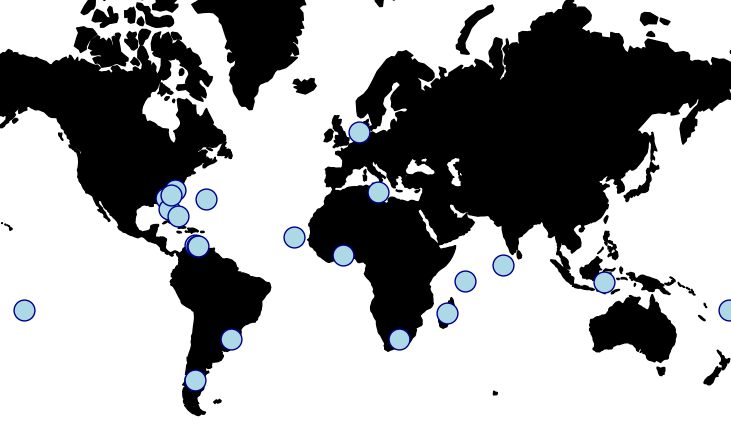
\includegraphics[width=\columnwidth]{Research_map/research_areas.png}



     \section[\faBook]{Publications}
     {\small I published \textbf{98 articles} in international scientific journals, \textbf{11 on other peer-reviewed media} and \textbf{6 book chapters and books}.} 
     \smallskip

    \section[\faUnlock]{Open data}
    {\small I share open-access datasets and presentations on the following platforms:}\\
    \faExternalLink \hspace{0.5em} \href{https://zenodo.org/search?page=1&size=20&q=creators.orcid:(0000-0001-5575-1168)&sort=mostrecent}{Zenodo}\\
    \faExternalLink \hspace{0.5em} \href{https://www.pangaea.de/?q=Rovere\%2C+Alessio&f.author\%5B\%5D=Rovere\%2C+Alessio}{PANGAEA}\\
    \faExternalLink \hspace{0.5em} \href{https://figshare.com/authors/Alessio_Rovere/1379355}{Figshare}


}

\mainbar{  

\section[\faEuro]{Funding}
{\normalsize \textbf{Research projects} -  As \textbf{Principal Investigator}, I have successfully led several research projects, securing a total of \textbf{~4.2 million \texteuro} in funding. In particular, I hold a Starting Grant from the European Research Council (ending in 2025), and I started my own research group at the University of Bremen and at the Leibniz Center for Tropical Marine Research thanks to funding of the German Science Foundation. I have participated in several research projects as \textbf{Co-Principal Investigator}, for a total amount of \textbf{960 thousand \texteuro}.\\
\textbf{Conferences and workshops} - I have played a significant role in organizing conferences and workshops, directly managing funds provided by various associations and institutions to cover expenses and support the participation of \textbf{young scientists and scientists from low-income or developing countries}. I have contributed to grant writing and the management of funds. Overall, since 2012 I secured \textbf{\textasciitilde55 thousand \texteuro} from scientific associations such as PAGES, INQUA and the EGU.
}

\section[\faInstitution]{Academic service}
\subsection{Academic service}
\achievement{\textbf{Since 2024.} Coordinator of the degree course (MSc and BSc) in Environmental Sciences at Ca' Foscari University of Venice}
\achievement{\textbf{Since 2023.} President of the "Coastal and Marine Processes" commission of the International Union for Quaternary Sciences} 
\achievement{\textbf{Since 2023.} Ph.D. Program Board (Collegio di dottorato) for the "Doctoral of National Interest in Polar Sciences" at Ca’ Foscari University of Venice} 
\achievement{\textbf{Since 2022.} Member of the Steering Committee of the "Instabilities and Thresholds in Antarctica (INSTANT) of SCAR}  
\achievement{\textbf{Since 2022.} Member of the "Ca' Foscari ERC Board"} 
\achievement{\textbf{Since 2022.} Member of the "ESAlab" Scientific Committee (Ca' Foscari and European Space Agency)} 
\achievement{\textbf{Since 2022.} Member of the "Technical and Scientific Commitee" of the Cinque Terre Marine Protected Area (IT)} 
\achievement{\textbf{2020.} Contributing author for the 6th Assessment Report of the Intergovernmental Panel on Climate Change} 
\achievement{\textbf{2018-2023.} Co-leader of the International working group ‘PALSEA’ PALeo constraints on SEA level rise, funded by PAGES and INQUA} 
\achievement{\textbf{2012-2016.} Co-leader of the International working group ‘MEDFLOOD’, sponsored by INQUA} 

\subsection{Editor / reviewer roles}
\achievement{\textbf{Since 2022.} Journal editor - Earth System Science Data, Copernicus (EGU, Since 2022) and Climate of the Past, Copernicus (EGU, Since 2018)}
\achievement{\textbf{2019-2022.} Book editor - Book: UAVs in Environmental Sciences}
\achievement{\textbf{2019-2022.} Special Issue Editor - Earth System Science Data and Quaternary Science Reviews}
\achievement{\textbf{Since 2012.} Reviewer for more than 50 manuscripts and for research proposals to several international foundations}

\subsection{Conferences, workshops and convened sessions}
\achievement{\textbf{2023.} Convener and session chair at several conferences (INQUA  Rome - 2023, PAGES OSM - 2022, GeoBremen - 2017, AGU - 2015} 
\achievement{\textbf{2017 to 2022.} Co-organizer of the annual PALSEA workshop (2017, Galloway, NJ, USA - 2019, Dublin, IE - 2020, Online - 2022, Singapore)}
\achievement{\textbf{2021-2022.} Co-organizer of a webinar series on paleo sea level organised jointly by PALSEA, WCRP (sea level), IAG, and SERCE} 
\achievement{\textbf{2019.} Co-organizer of the CoChE Summer school. Coastal Changes and Evolution. Oristano, IT} 
\achievement{\textbf{2012 to 2016.} Co-organizer of the annual MEDFLOOD workshop (2012, Rome, IT - 2014, Haifa, IL - 2016, Bremen, DE)}

    
}      
\makebody

\clearpage

\pagestyle{empty}

\nocite{*}
\section[\faBook]{Selected publications}
The names of postdocs, Ph.D. or master students authored while under my mentoring or supervision are \underline{underlined}. A full publication list is available \href{https://github.com/Alerovere/Resume/blob/main/Resume_AR/Resume_full_ENG.pdf}{here \faExternalLink}

\printbibliography[heading=none]

\end{document}